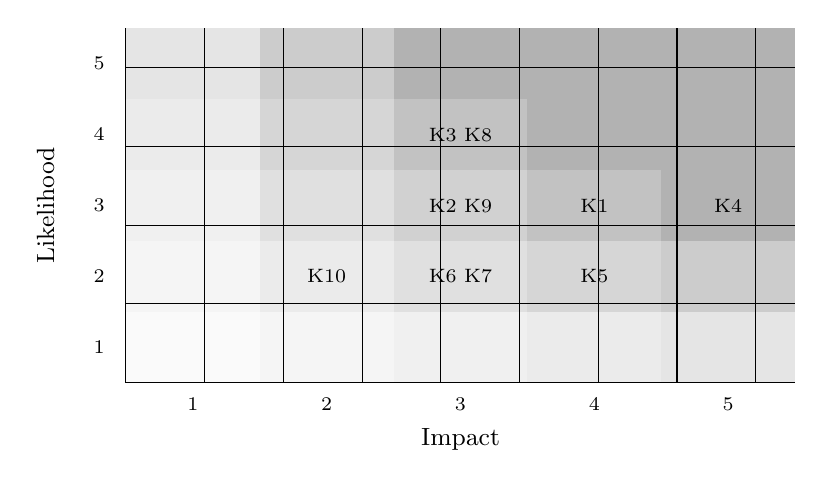
\begin{tikzpicture}[x=1.7cm, y=0.9cm]
\fill[gray!4] (0,0) rectangle (1,1);
\fill[gray!8] (1,0) rectangle (2,1);
\fill[gray!12] (2,0) rectangle (3,1);
\fill[gray!16] (3,0) rectangle (4,1);
\fill[gray!20] (4,0) rectangle (5,1);
\fill[gray!8] (0,1) rectangle (1,2);
\fill[gray!16] (1,1) rectangle (2,2);
\node[font=\scriptsize] at (1.5,1.5) {K10};
\fill[gray!24] (2,1) rectangle (3,2);
\node[font=\scriptsize] at (2.5,1.5) {K6 K7};
\fill[gray!32] (3,1) rectangle (4,2);
\node[font=\scriptsize] at (3.5,1.5) {K5};
\fill[gray!40] (4,1) rectangle (5,2);
\fill[gray!12] (0,2) rectangle (1,3);
\fill[gray!24] (1,2) rectangle (2,3);
\fill[gray!36] (2,2) rectangle (3,3);
\node[font=\scriptsize] at (2.5,2.5) {K2 K9};
\fill[gray!48] (3,2) rectangle (4,3);
\node[font=\scriptsize] at (3.5,2.5) {K1};
\fill[gray!60] (4,2) rectangle (5,3);
\node[font=\scriptsize] at (4.5,2.5) {K4};
\fill[gray!16] (0,3) rectangle (1,4);
\fill[gray!32] (1,3) rectangle (2,4);
\fill[gray!48] (2,3) rectangle (3,4);
\node[font=\scriptsize] at (2.5,3.5) {K3 K8};
\fill[gray!60] (3,3) rectangle (4,4);
\fill[gray!60] (4,3) rectangle (5,4);
\fill[gray!20] (0,4) rectangle (1,5);
\fill[gray!40] (1,4) rectangle (2,5);
\fill[gray!60] (2,4) rectangle (3,5);
\fill[gray!60] (3,4) rectangle (4,5);
\fill[gray!60] (4,4) rectangle (5,5);
\draw (0,0) grid (5,5);
\foreach \n in {1,...,5} {
  \node[font=\scriptsize] at (\n-0.5,-0.3) {\n};
  \node[font=\scriptsize] at (-0.2,\n-0.5) {\n};
}
\node[font=\small] at (2.5,-0.8) {Impact};
\node[font=\small, rotate=90] at (-0.6,2.5) {Likelihood};
\end{tikzpicture}
